\documentclass[a4paper]{article}

\usepackage[utf8]{inputenc}

\usepackage{csquotes}

\usepackage[
    backend=biber,
    style=authoryear-icomp,
    natbib=true,
    url=false,
    doi=true,
    eprint=false
]{biblatex}

%\addbibresource{references.bib}

\def\constantMaxdrawdown{42.0}
\def\constantStartdate{1999-11-01 00:00:00}
\def\constantEnddate{2025-01-29 00:00:00}
\def\constantTransactionCommission{0.02}
\def\constantRMean{0.0026}
\def\constantSharpeRatio{0.4906}
\def\constantStd{0.0053}

\usepackage{graphicx}
\usepackage{float}
\usepackage{amsmath}
\usepackage[english]{babel}
\usepackage[bookmarks=true]{hyperref}

\def\documenttitle{Description of Bot Tau}

\title{\documenttitle}
\date{\today}
\author{Frans Englich \\
        \href{mailto:fenglich@fastmail.fm}{fenglich@fastmail.fm}}

\hypersetup{
    pdfsubject = {\documenttitle},
    pdftitle = {\documenttitle}
}

\begin{document}

\maketitle

This document documents the simulated in-sample performance of Bot Tau's trading
strategy. It does not document the strategy itself, which is proprietary.

\section{Drawdown}

Maximum drawdown is \constant_maxdrawdown \%.

\begin{figure}
    \begin{center}
        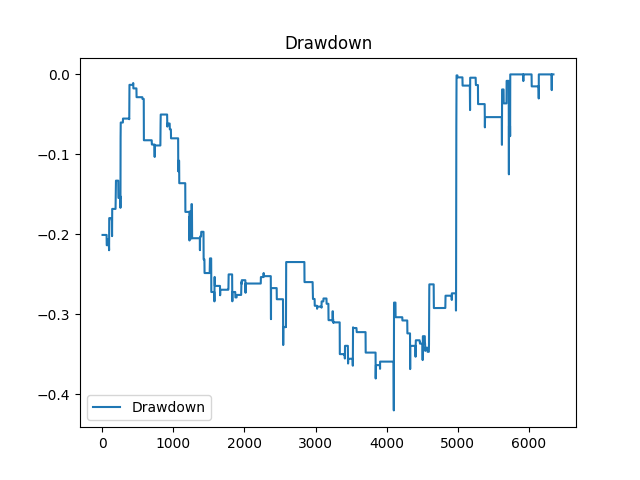
\includegraphics{../generated/drawdown.png}
    \end{center}
    %\caption{}
\end{figure}

%\printbibliography
%\appendix

\end{document}
